% Metódy inžinierskej práce

\documentclass[10pt,twocolumn,twoside,slovak,a4paper]{article}

\usepackage[slovak]{babel}
%\usepackage[T1]{fontenc}
\usepackage[T1]{fontenc} % lepšia sadzba písmena Ľ než v T1
\usepackage[utf8]{inputenc}
\usepackage{graphicx}
\usepackage{url} % príkaz \url na formátovanie URL
\usepackage{hyperref} % odkazy v texte budú aktívne (pri niektorých triedach dokumentov spôsobuje posun textu)
\usepackage{todonotes}
\usepackage{cite}
\usepackage{fancyhdr}
\usepackage{wrapfig}
\usepackage{stfloats}
%\usepackage{times}

\pagestyle{fancy}
\fancyhead{}



\title{Je odporúčací systém Netflix-u problém ?\thanks{Semestrálny projekt v predmete Metódy inžinierskej práce, ak. rok 2024/2025, vedenie: Mgr. Yevheniia Kataieva, PhD.}}

\author{Adam Glogovský\\[2pt]
	{\small Slovenská technická univerzita v Bratislave}\\
	{\small Fakulta informatiky a informačných technológií}\\
	{\small \texttt{xglogovsky@stuba.sk}}}

\date{\small 5. október 2024} 



\begin{document}

\maketitle

\section*{Abstract}
% \begin{center}
% 	\textbf{Abstract}
% \end{center}
% \vspace{0.5em}
% \noindent
Touto prácou by som chcel poukázať na to, ako Netflix ako firma spracúva užívateľské informácie a či je to správne. Na začiatku tejto práce objasním problematiku všeobecných odporúčacích systémov. Potom ukážem kde Netflix posiela užívateľské informácie. Ako ich spracúva a ako podľa nich dokáže nám užívateľom spríjemniť fungovanie na platforme. Ak nám to zvyšuje zážitok z používania tejto platformy, čo to teda tú platformu stojí a či je to vo výsledku pre danú platformu efektívne a finančne prospešné. Taktiež sa pokúsim čo naviac priblížiť samotné spracovanie týchto údajov a poukážem na to, či je správne daným spôsobom spracúvať tieto informácie.\cite{amatriain2015recommender}
\begin{figure*}[h]
	\centering
	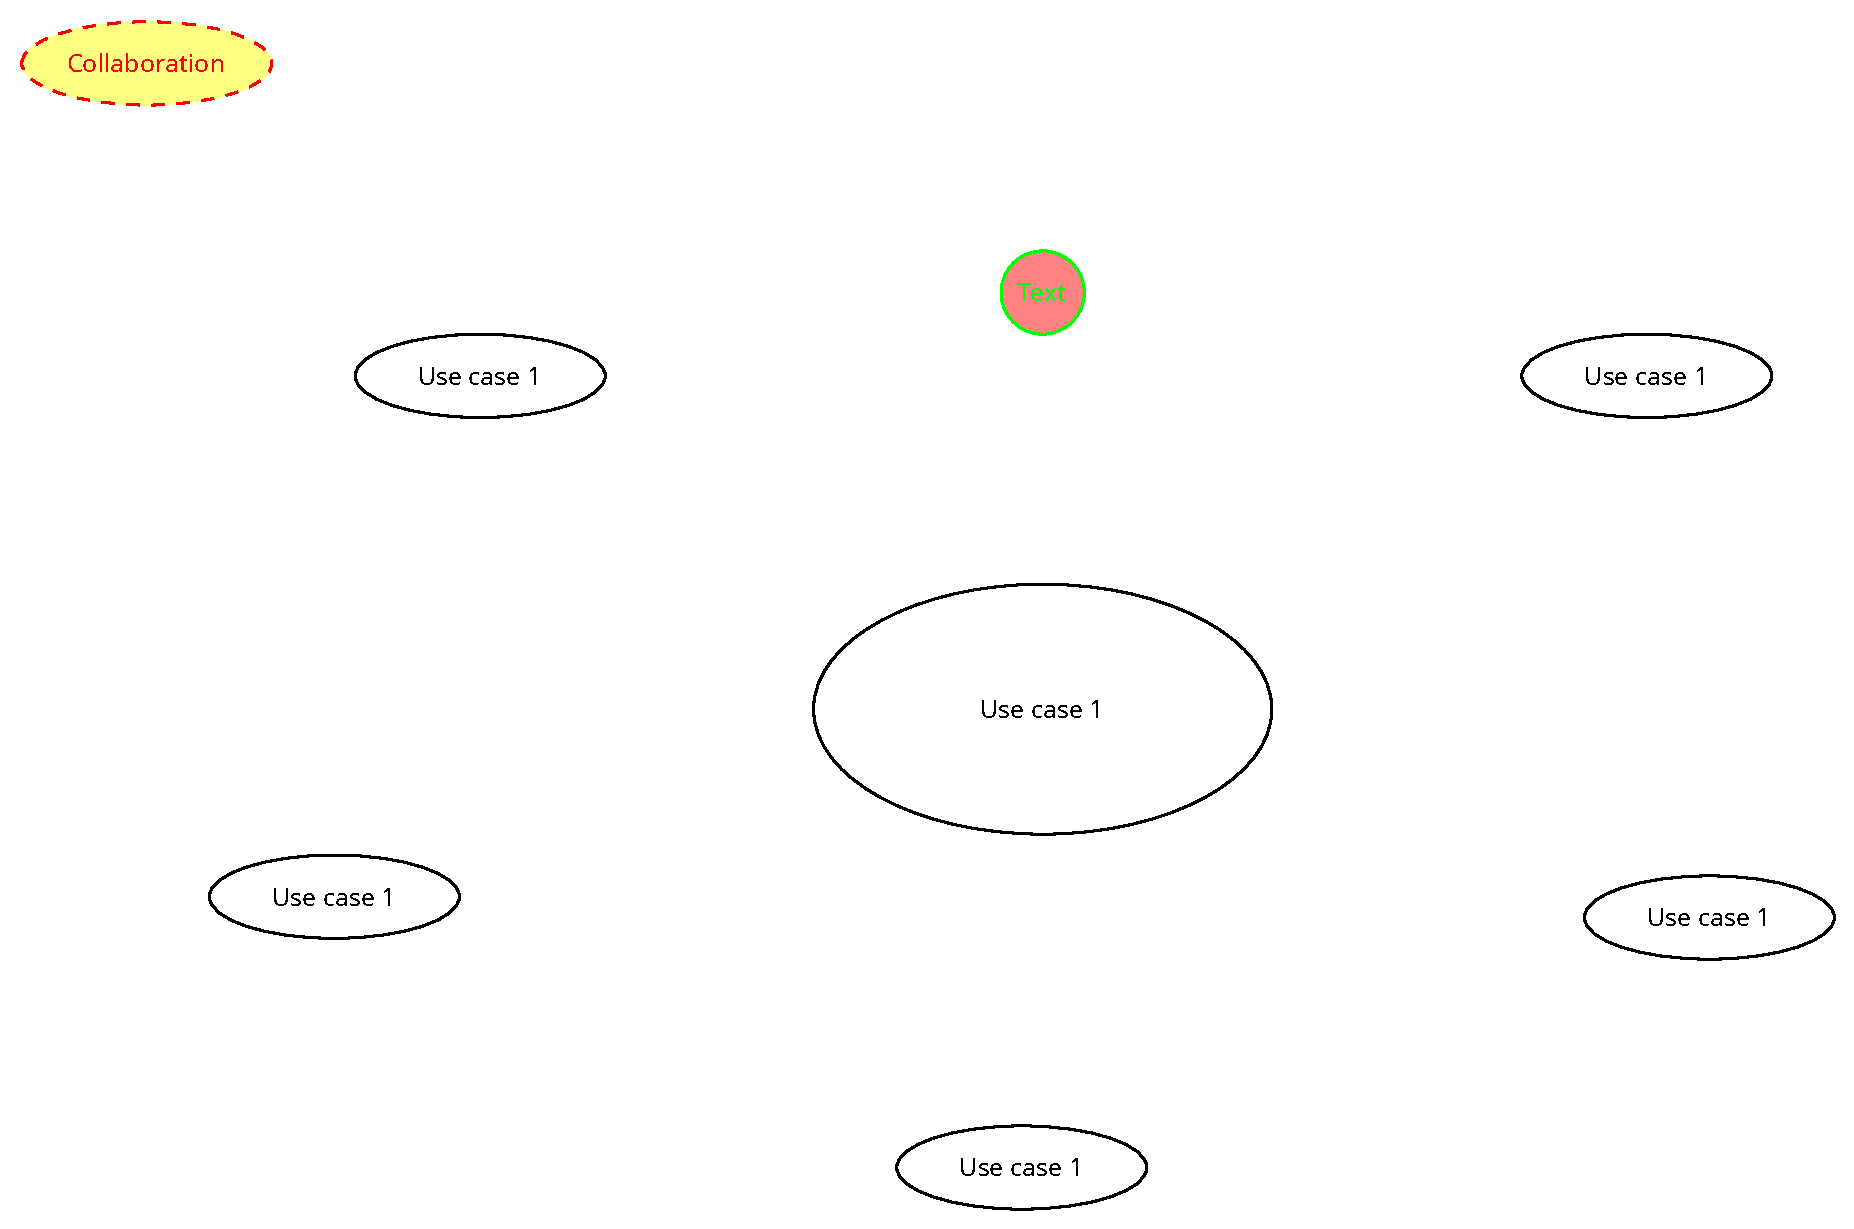
\includegraphics[scale=0.2]{diagram.pdf}
\end{figure*}
Dôležítý taktiež pre platformu je, algoritmus akým spracúvajú dané informácie a samotná infraštruktúra v ktorej to celé funguje. Samozrejme touto prácou chcem zistiť, či kvôli tomuto alogritmu a spôsobu spracovania informácií, Netflix neubližuje menej populárnemu alebo menej ''mainstream'' obsahu, ktorý je teda ešte o to menej ukazovaný užívateľom. A tiež poukážem na to, či je tento menej populárny obsah iba nefavoritizovaný a posúvaný nižšie v hľadaní, alebo je kompletne zahaľovaný určitým užívateľom. Na konci tejto práce teda budete vedieť ako Netflix spracúva informácie, či je správne spracovávať užívateľské informácie týmto spôsobom, či je to profitabilné pre Netflix a taktiež, či to prospieva užívateľom tejto platformy.\todo{204 slov}
Lorem ipsum dolor sit amet, consectetur adipiscing elit. Sed scelerisque a metus in fermentum. Curabitur hendrerit velit vel tortor condimentum malesuada. Donec vel tincidunt ex. Suspendisse finibus tortor in arcu aliquam faucibus. Fusce consectetur gravida quam a tincidunt. Duis tempor, nisi id ultrices porta, lorem leo vestibulum lacus, eu sagittis ex erat quis justo. Mauris eu magna felis. Aenean vehicula quis enim eget maximus. Quisque pharetra id libero vitae tristique. Proin ut bibendum elit. Praesent at ligula vitae augue auctor gravida. Cras pretium mollis lacus quis sodales. Fusce interdum massa elementum, vulputate odio id, molestie nibh.

Cras eu rutrum sem. Quisque pellentesque eget massa ac pellentesque. Nunc molestie pharetra dui eu aliquam. Vestibulum viverra, nulla nec eleifend ornare, nulla sapien scelerisque risus, quis auctor ligula purus tempor magna. Quisque imperdiet ex sed ultricies vulputate. Maecenas fermentum justo sed elementum pharetra. Vestibulum id ante elit. Mauris massa ipsum, fringilla quis consectetur blandit, cursus non massa. Sed pretium risus ut erat facilisis, non lacinia metus consectetur. Nulla aliquam metus luctus urna laoreet tincidunt. Aliquam luctus mattis ultrices. Maecenas tempus justo eu velit eleifend pellentesque eu mollis justo. Donec suscipit sapien erat, viverra placerat dui ultricies ut. Mauris eget velit a ex mollis faucibus in lobortis tellus.
Quisque quis lorem ac nibh ornare consequat vitae quis lectus. Vestibulum nec lectus eget nisi eleifend pharetra. Proin interdum mi tempus, posuere nisl eu, finibus tellus. Aenean fermentum semper commodo. Aliquam at augue mi. Nulla eu metus nec felis mollis malesuada. Nunc ac elit sollicitudin, commodo sapien nec, maximus massa. Proin ut lectus vel eros lacinia porttitor. Aliquam et pharetra felis, a sagittis tortor.Lorem ipsum dolor sit amet, consectetur adipiscing elit. Sed scelerisque a metus in fermentum. Curabitur hendrerit velit vel tortor condimentum malesuada. Donec vel tincidunt ex. Suspendisse finibus tortor in arcu aliquam faucibus. Fusce consectetur gravida quam a tincidunt. Duis tempor, nisi id ultrices porta, lorem leo vestibulum lacus, eu sagittis ex erat quis justo. Mauris eu magna felis. Aenean vehicula quis enim eget maximus. Quisque pharetra id libero vitae tristique. Proin ut bibendum elit. Praesent at ligula vitae augue auctor gravida. Cras pretium mollis lacus quis sodales. Fusce interdum massa elementum, vulputate odio id, molestie nibh.

Cras eu rutrum sem. Quisque pellentesque eget massa ac pellentesque. Nunc molestie pharetra dui eu aliquam. Vestibulum viverra, nulla nec eleifend ornare, nulla sapien scelerisque risus, quis auctor ligula purus tempor magna. Quisque imperdiet ex sed ultricies vulputate. Maecenas fermentum justo sed elementum pharetra. Vestibulum id ante elit. Mauris massa ipsum, fringilla quis consectetur blandit, cursus non massa. Sed pretium risus ut erat facilisis, non lacinia metus consectetur. Nulla aliquam metus luctus urna laoreet tincidunt. Aliquam luctus mattis ultrices. Maecenas tempus justo eu velit eleifend pellentesque eu mollis justo. Donec suscipit sapien erat, viverra placerat dui ultricies ut. Mauris eget velit a ex mollis faucibus in lobortis tellus.

Quisque quis lorem ac nibh ornare consequat vitae quis lectus. Vestibulum nec lectus eget nisi eleifend pharetra. Proin interdum mi tempus, posuere nisl eu, finibus tellus. Aenean fermentum semper commodo. Aliquam at augue mi. Nulla eu metus nec felis mollis malesuada. Nunc ac elit sollicitudin, commodo sapien nec, maximus massa. Proin ut lectus vel eros lacinia porttitor. Aliquam et pharetra felis, a sagittis tortor.

%\begin{wrapfigure}{r}{0.5\textwidth}

%\end{wrapfigure}


\begin{figure}
	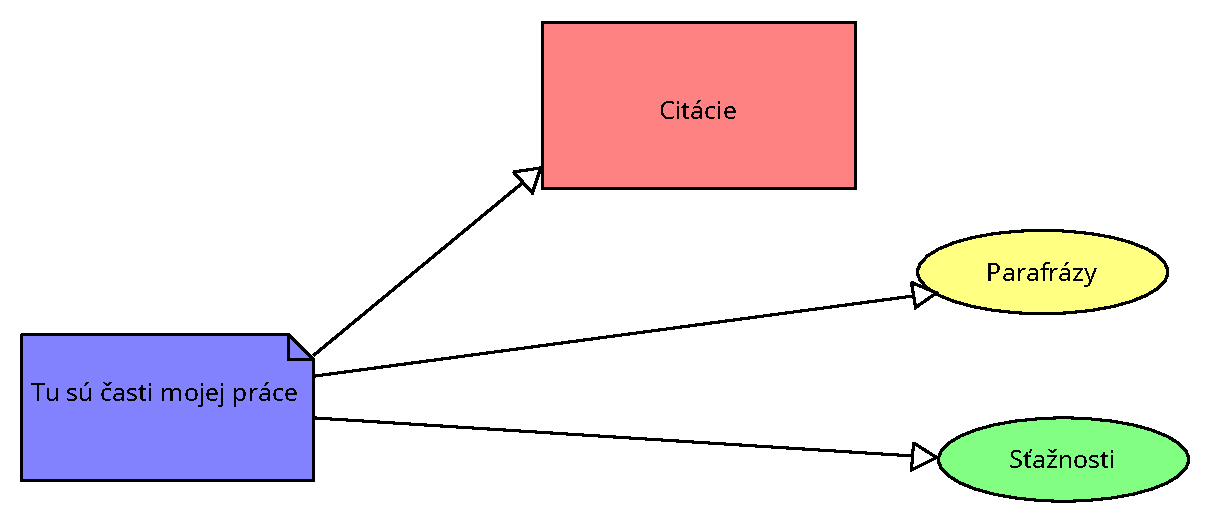
\includegraphics[scale=0.4]{diagram horizontal.pdf}
\end{figure}




\newpage

%\acknowledgement{Ak niekomu chcete poďakovať\ldots}


% týmto sa generuje zoznam literatúry z obsahu súboru literatura.bib podľa toho, na čo sa v článku odkazujete
\begin{figure}
	\bibliography{literatura}
	\bibliographystyle{abbrv} % prípadne alpha, abbrv alebo hociktorý iný
\end{figure}

\end{document}
